\graphicspath{
  {./images/bmps/}{./images/vects/}{./images/}
  {./images/presentation/bmps/}{./images/presentation/vects/}{./images/presentation/}
  {./images/chapter00/bmps/}{./images/chapter00/vects/}{./images/chapter00/}
  {./images/chapter03/bmps/}{./images/chapter03/vects/}{./images/chapter03/}
}

\subsection{Evaluation of Stereo 3D Reconstruction Algorithms}
\begin{frame}{Introduction}
 REVISAR!!!! Usar la versión pptx
\end{frame}

\begin{frame}{Introduction}
  \begin{itemize}
    \item We want to know the best performance algorithms available for environmental mapping.
    \item Very few datasets $\rightarrow$ Most of them in controlled conditions
    \item Three different dense reconstruction algorithm implementations
    \item Three different and well-known evaluation strategies
  \end{itemize}
  
  \note {
  \begin{itemize}
   \item Critical tasks in the development of driving assistance systems and stereo vision has been widely used to accomplish it
   \item that allow assessing the performance of a specific method in a real world application
   \item conditions... which are not able to capture the variety of the real world
   \item These strategies represent a trade-off btween cost, set up time and accuracy
  \end{itemize}
  }
\end{frame}

\begin{frame}{Introduction}
  Little o no data available to be used as ground truth.
  \begin{itemize}
    \item<1-> Use of a high-end LIDAR (LIgth Detection and Ranging) unit.
    \item<2-> Exploit a prior over the data-set.
    \item<3-> Synthesize a virtual view
  \end{itemize}
  \begin{overlayarea}{\textwidth}{\textheight}
    \only<2>{
    \begin{exampleblock}{Example}
      The presence of freespace in front of a manually driven vehicle to detect wrongly reconstructed points.
    \end{exampleblock}
    }
    \only<3>{
    \begin{exampleblock}{Example}
      A virtual view synthesized from the reconstructed environment geometry can be compared with the actual data recorded from a third camera.
    \end{exampleblock}
    }
  \end{overlayarea}
  
  \note {
  }
\end{frame}

\begin{frame}{Experimental setup}
  \begin{itemize}
    \item<1-> Van set up to take part to the VisLab Intercontinental Autonomous Challenge (VIAC).
    \item<2-> Point Grey Bumblebee XB3-13S2C color camera.
    \item<3-> SICK LD-MRS-400001.
  \end{itemize}
  \only<1->{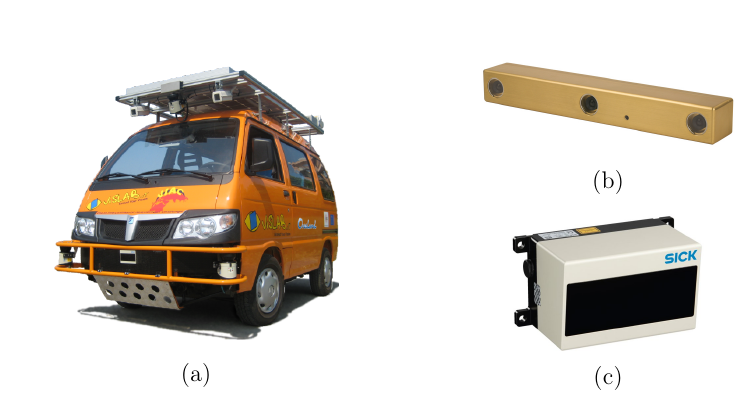
\includegraphics[width=\textwidth, trim=0 0 0 40,clip]{viac}}
  \vskip-5.5cm
  \begin{overlayarea}{0.5\textwidth}{\textheight}
    \only<2>{
    \begin{block}{Bumblebee XB3-13S2C}
      \begin{itemize}
       \item 3.5\,mm optics.
       \item $1280\times960$\,pixels.
      \end{itemize}
    \end{block}
    }
    \only<3>{
    \vskip 2cm
    \begin{block}{SICK LD-MRS-400001}
      \begin{itemize}
       \item 4 planes.
       \item 12.5\,Hz
       \item Angular resolution: 0.125$^\circ$.
       \item Field of View: 85$^\circ$.
      \end{itemize}
    \end{block}
    }
  \end{overlayarea}
  
  \note {
  
  }
\end{frame}